


\chapter{Realisierung }

	\begin{figure}[H]
		\centering
		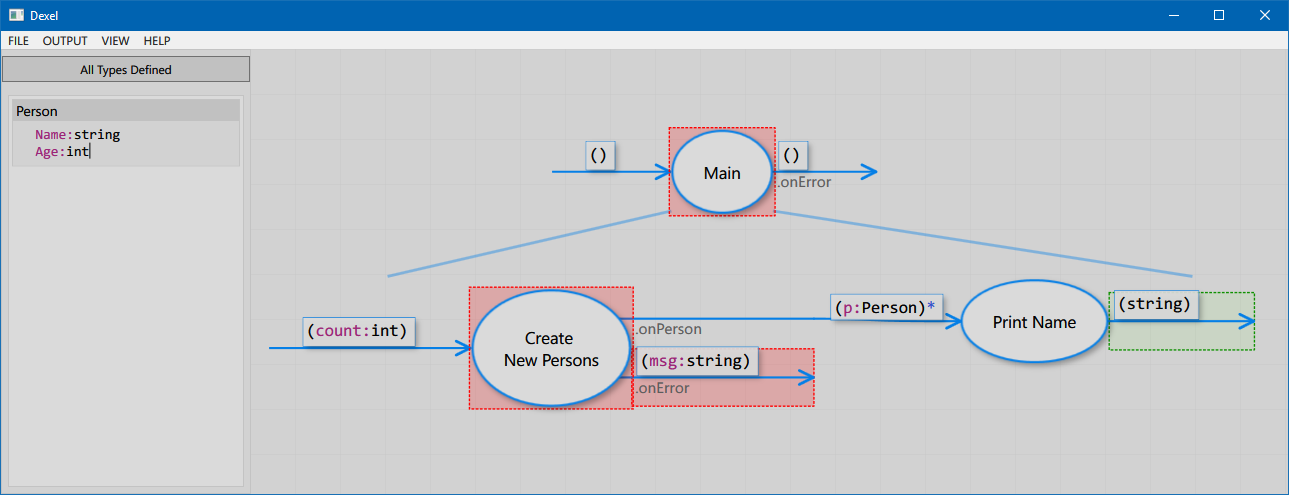
\includegraphics[width=1\linewidth]{./img/Dexel.png} 
		\caption{Dexel}
	\end{figure}


In diesem Kapitel soll vorgestellt werden, was in dem Zeitraum dieser
Bachelorarbeit erreicht wurde. Die Architektur der Anwendung wurde selbst nach
Flow Design umgesetzt und bietet somit dem Leser eine Quelle an weiteren
konkreten Beispielen, wie eine Methode nach IOSP in der Praxis aussieht.

Als Arbeitstitel für die Anwendung wurde der Name Dexel gewählt.

\section{Übersicht über die unterschiedlichen Projekte}




Die Anwendung besteht aus einer \textit{Solution}, die folgende Unterprojekte beinhaltet\footnote{Bei komplexen Funktionalitäten wurde nach TDD (Test Driven Development)
	programmiert, bei dem zuerst der Test geschrieben wird, der das zu erwartende
	Ergebnis definiert, und erst anschließend die Methode implementiert wird. Diese Tests wurden in einem extra Test-Projekt für jedes Projekt zusammengefasst.}: 
	\begin{figure}[H]
		\centering
		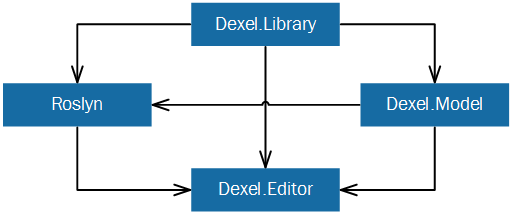
\includegraphics[width=0.8\linewidth]{./img/Projekte.png} 
		\caption{Aufbau der Assembly-Struktur und Abhänigkeiten zwischen den Dexel-Unterprojekten}
	\end{figure}



\subsubsection{Dexel.Model / Dexel.Model.Tests}

Dieses Projekt beinhaltet das Domänenmodell - alle Datentypen die zur internen Repräsentation
eines Flow Design Diagramms nötig sind. Außerdem beinhaltet dieses Projekt
statische Manager-Klassen, die das Arbeiten mit den Datentypen vereinfachen.

\subsubsection{Dexel.Editor / Dexel.Editor.Tests}

Dies ist das Hauptprojekt, das alle anderen Projekte integriert.
Nach Flow Design kann man IOSP auf Projekt-Ebene anwenden, hier wurde jedoch das IOSP
Prinzip nicht eingehalten. Dieses Projekt hat nicht nur die Aufgabe die
anderen Projekte zu integrieren, sondern beinhaltet selbst den
UI-Sourcecode. Diese Entscheidung wurde gefällt, da ein Extrahieren der UI
in ein anderes Projekt sich als zu schwierig erwies. Eine Lösung dafür zu
finden, wie ein Event aus dem UI mit einer Funktionalität verbunden werden
könnte, dass sich in einem Projekt befindet, war zeitlich zu
aufwendig. Aus diesem Grund wurde entschieden auf die zusätzliche
Komplexität einer Entkoppelung zu verzichten und es einfacher zu halten, indem
dieses Projekt sowohl die UI beinhaltet, als auch alle anderen Projekte
kennt.

\subsubsection{Roslyn / Rosyln.Tests}

Diese Projekt beinhaltet die Logik zur Erstellung von C\#-Code aus einem Flow
Design. Mircosoft Rosyln ist die Technik, die hier zum Erstellen von Code zum
Einsatz kommt.
Das Flow Design Diagramm muss in Form eines \texttt{MainModels} aus dem
Dexel.Model Projekt vorliegen. Aus diesem Grund gibt es eine Abhängigkeit
zwischen diesem und dem Dexel.Model Projekt. 

Eine Trennung dieser Abhängigkeit wurde versucht umzusetzen indem gegen ein Interface
programmiert wurde, anstatt gegen die konkrete Implementation in
Dexel.Model. Diese Interfaces der Datentypen und Manager-Klassen wurde dann
in ein Contracts-Projekt ausgelagert, von dem alle anderen Projekte abhängig
sein durften. Die zusätzliche Komplexität, Mehraufwand und ein Problem bei
der Serialisierung von Datentypen, die Interfaces als Eigenschaften besaßen,
machte es nicht wert hier eine Entkoppelung zu schaffen. Somit wurde beschlossen die Änderung rückgängig zu machen und auf die Interfaces zu verzichten.

\subsubsection{Dexel.Library}

Dieses Projekt beinhaltet einige Methoden (meist Extension-Methoden), die ein Arbeiten
nach Flow Design erleichtern. Diese wurden in ein separates Projekt
ausgelagert, damit alle anderen Projekte darauf zugreifen können.

\section{Das Domänenmodell}

	\begin{figure}[H]
		\centering
		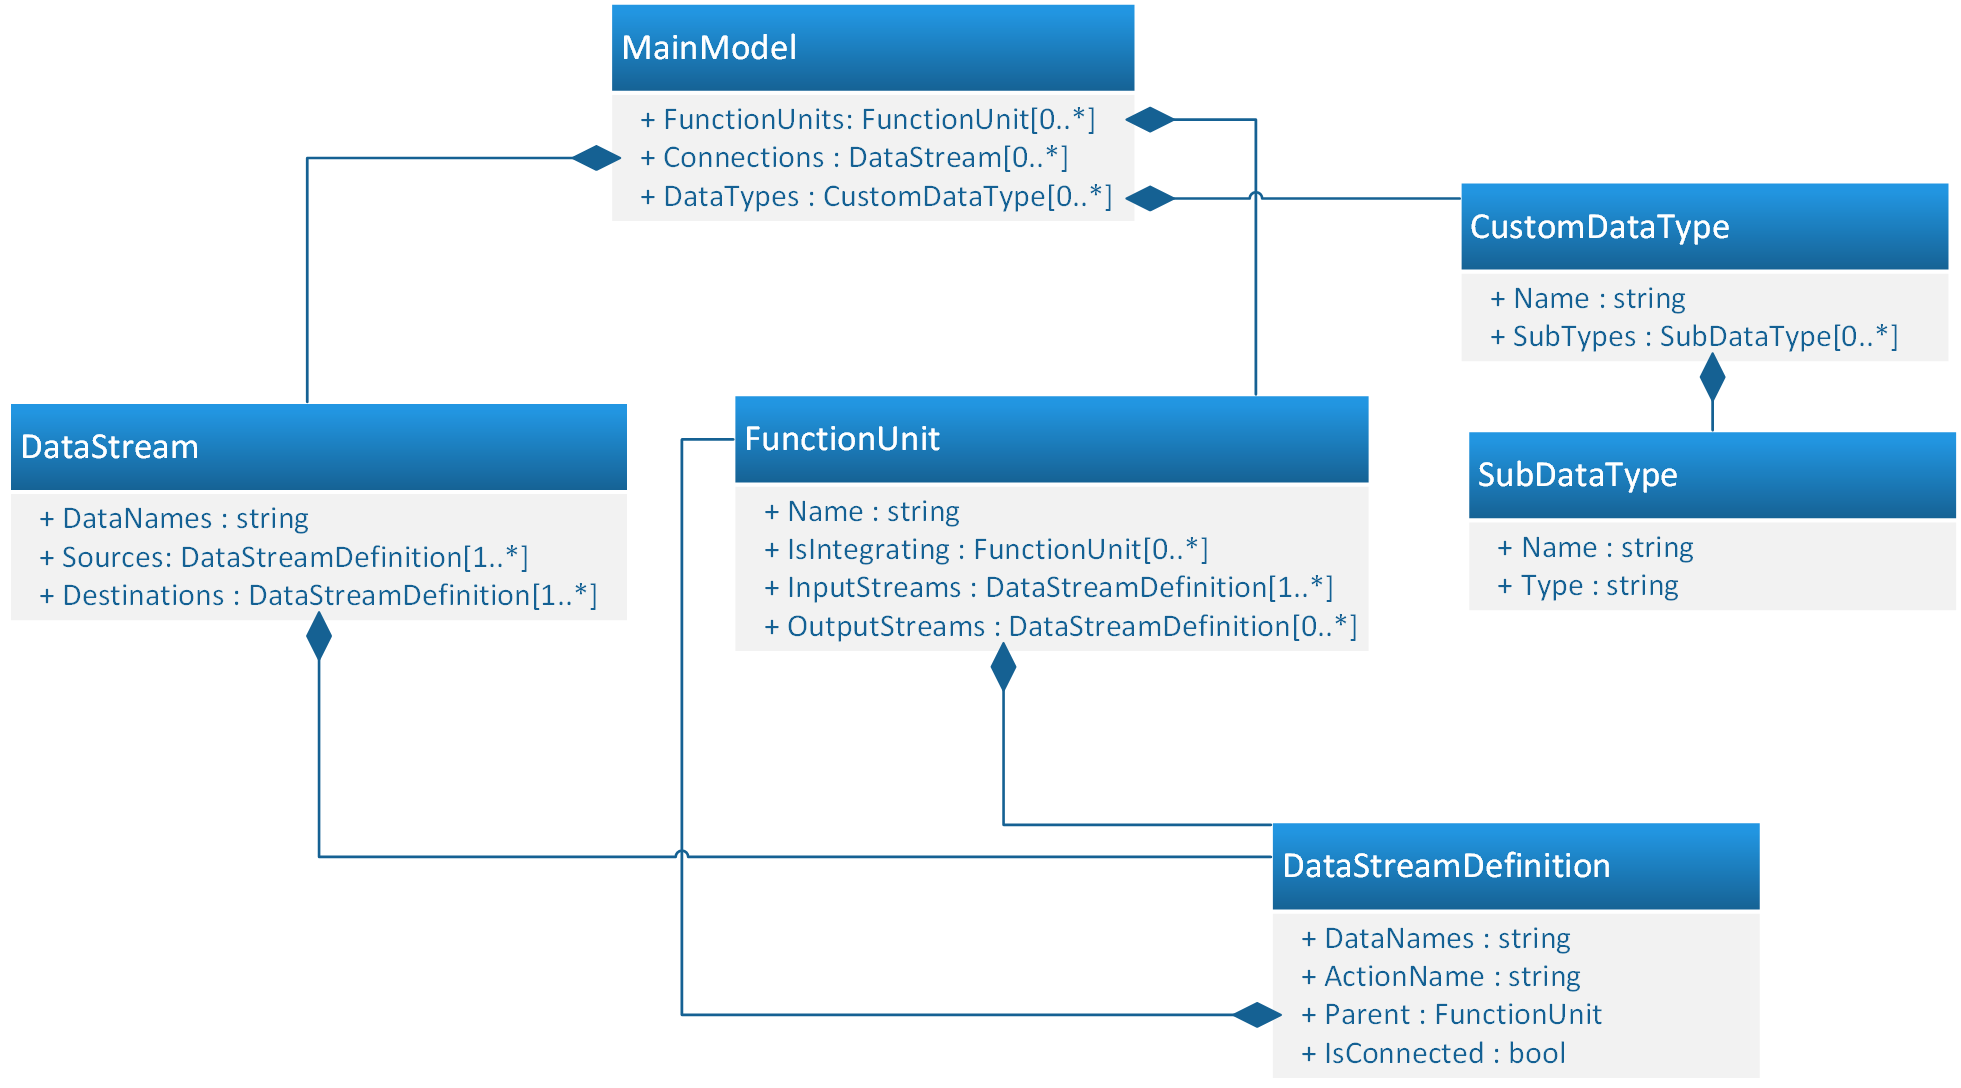
\includegraphics[width=1\linewidth]{./img/ModellUml.png} 
		\caption{Das Domänenmodell von Dexel}
	\end{figure}


Um nachfolgende Kapitel der Realisierung und die darin enthaltenden
Codeausschnitte verstehen zu können, braucht es ein Verständnis darüber, wie die
grundlegenden Datentypen des Domänenmodells aufgebaut sind. Um die Funktionalität der
jeweiligen Datentypen besser zu veranschaulichen, werden in diesem Kapitel
Bilder verwendet, welche die spätere Darstellung des Datentyps in der UI zeigen.

\subsubsection{MainModel}

Das \texttt{MainModel} ist, wie der Name schon sagt, das Haupt-Modell, das alle
anderen Modelle per Komposition beinhaltet. Somit kann einer Methode einfach eine Objektinstanz
eines \texttt{MainModels} übergeben werden und erhält dadurch alle Informationen über das aktuelle Flow-Design-Diagramm. 
Das \textit{MainModel} beinhaltet alle Funktionseinheiten, alle verbindenden
Datenströme (\textit{Connections}) und alle benutzerdefinierten Datentypen (\textit{DataTypes}).

	\subsubsection{FunctionUnit}
	
\begin{figure}[H]
	\centering
	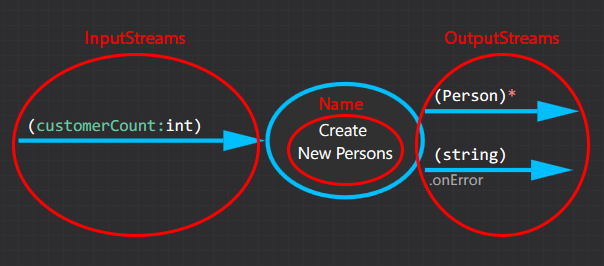
\includegraphics[width=0.9\linewidth]{./img/FunctionUnitView.png} 
	\caption{Dexel-Screenshot: FunctionUnit-View}
\end{figure}

Die \texttt{Name}-Eigenschaft ist der Name der Funktionseinheit (der Text, der bei der
Darstellung später innerhalb des Kreises erscheint). Dieser wird später per \textit{Binding}
direkt an die UI gebunden. 

Die \texttt{IsIntegrating}-Eigenschaft gibt an, ob diese Funktionseinheit eine Integration
ist und welche andere Instanzen von Funktionseinheiten sie integriert.
Eine leere Liste besagt, dass die Funktionseinheit keine Integration ist.

Die \texttt{Input}- und \texttt{OutputStreams} definieren die möglichen ein- und ausgehenden
Datenströme der Funktionseinheiten. An diese \texttt{DataStreamDefinitionen} können sich \\\texttt{DataStreams}
verbinden. Dadurch lassen sich die Datenflüsse modellieren.


	\subsubsection{DataStreamDefinition}

	
		
		\begin{figure}[H]
			\centering
			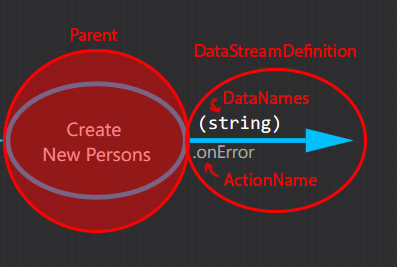
\includegraphics[width=0.6\linewidth]{./img/DataStreamDefinitionView.png} 
			\caption{Dexel-Screenshot: DataStreamDefinition-View}
		\end{figure}
	
	Eine Funktionseinheit verfügt über ein oder mehrere ein- und ausgehende
	\\\texttt{DataStreamDefinitionen}. Diese können verbunden sein oder nicht. Wenn eine
	Verbindung erstellt und gelöscht wird, muss deshalb auch die \texttt{Connected}-Eigenschaft
	immer angepasst werden, damit das Modell valide bleibt.
	Ob eine \texttt{DataStreamDefinition} verbunden ist, oder nicht, ist später
	für die Darstellung relevant.
	Eine \texttt{DataStreamDefinition} kennt auch die Funktionseinheit, von der sie ein
	Ein- oder Ausgang ist.
	
	Eine weitere grundlegende Eigenschaft ist die Benennung der Daten, die auf dem
	Datenfluss fließen. Für Ausgänge ist auch die Angabe eines
	Names manchmal nötig. Dieser soll später unterhalb des Pfeiles
	dargestellt werden.

\subsubsection{DataStream (Connections)}

Um Datenflüsse zwischen Funktionseinheiten zu beschreiben, bedarf es einer
Verbindungsklasse. Die DataStream-Klasse stellt diese Verbindungsklasse dar.



		\begin{figure}[H]
			\centering
			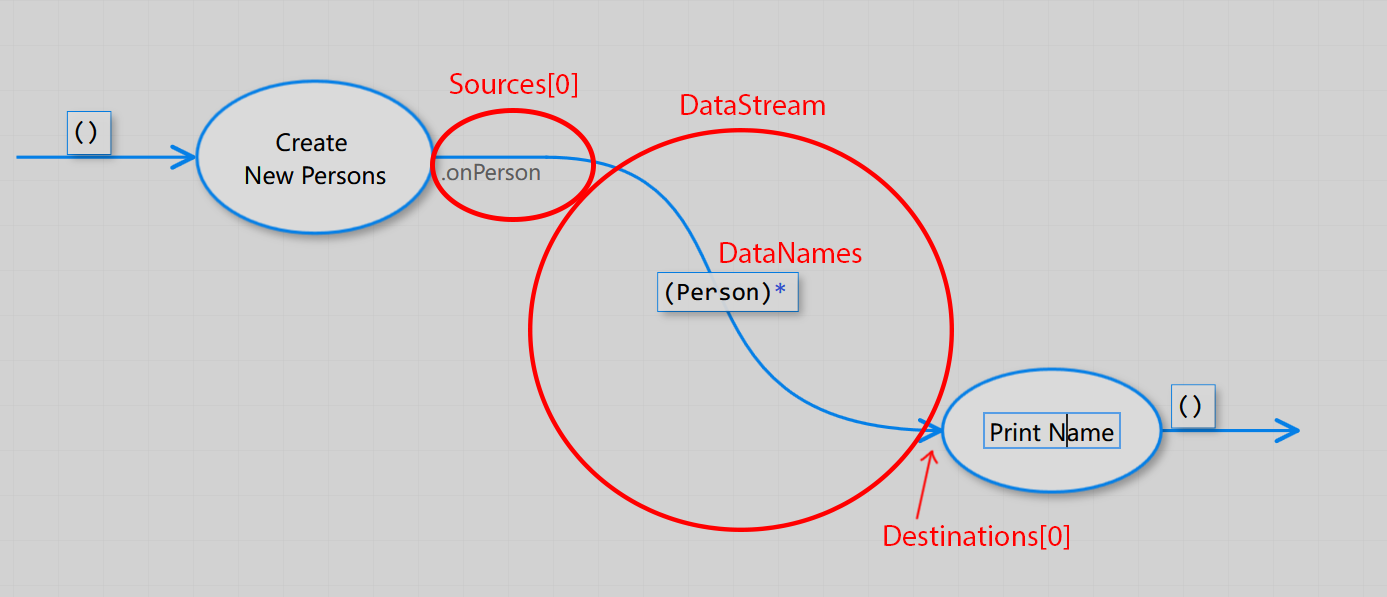
\includegraphics[width=0.9\linewidth]{./img/DataStreamView.png} 
			\caption{Dexel-Screenshot: DataStream-View}
		\end{figure}


Ein \texttt{DataStream} hat ein oder mehrere Referenzen an \texttt{DataStreamDefinition} als
Quellen und ein oder mehrere Referenzen an \texttt{DataStreamDefinition} als Ziele.
Um ein Datenstrom zu beschreiben, der aus mehren Quellen Daten bezieht und
an einer Stelle zusammenläuft, wird ein \texttt{DataStream} benötigt, der mehrere
Einträge in der \texttt{Source}-Liste besitzt und ein Eintrag in der
\texttt{Destination}-Liste. Dieser Datenstrom wäre dann ein Joined Input.
Ein Datenstrom mit einer Quelle und mehreren Zielen wäre ein sog. Split.

Die \texttt{DataNames}-Eigenschaft beinhaltet den Text, der später in der Mitte des
Pfeiles dargestellt werden soll. Eine Änderung dieser Eigenschaft bedarf
einer Aktualisierung der \texttt{DataNames} aller \texttt{Sources} und \texttt{Destinations}.
Die Aktualisierungsmethode muss die optionalen Pipe-Notation kennen und
entsprechend dieser die Ein- und Ausgänge aktualisieren.

Der aktuelle Stand der UI kann nur Datenflüsse mit einer Quelle und
einem Ziel darstellen.

\subsubsection{DataType}


\begin{figure}[H]
	\centering
	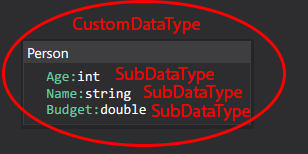
\includegraphics[width=0.5\linewidth]{./img/CustomDataType.png} 
	\caption{Dexel-Screenshot: CustomDataType-View}
\end{figure}


Ein benutzerdefinierter Datentyp besteht aus einem Namen und einer Liste von mehreren
\texttt{SubDataType}-Objekten. 

Ein \texttt{SubDataType} besteht aus einem Namen und den Namen
des Typen (zum Beispiel \texttt{string}, \texttt{int} oder auch ein anderen benutzerdefinierten Datentyp).

\subsubsection{Manager-Klassen}

\begin{enumerate}
	\item\texttt{MainModelManager}
	
	Einer der relevantesten Manager-Klassen ist die \texttt{MainModelManager}-Klasse,
	diese stellt die wichtigsten Funktionalitäten zur Verfügung die mit dem
	Arbeiten des \texttt{MainModels} gebraucht werden. Einige dieser Funktionalitäten
	wären: Verbinden und Trennen von Funktionseinheiten, vorwärts und rückwärts
	Traversieren entlang des Graphen, Hinzufügen und Entfernen einer
	Funktionseinheit von einer Integration, Hinzufügen, Löschen und Duplizieren
	von Funktionseinheiten, oder Teile des Graphen.
	
	\item\texttt{DataStreamManager}
	
	Diese statische Klasse bietet einige Funktionalitäten, die das Arbeiten mit
	Objekten der DataStream-Klasse vereinfachen soll.
	
	Ein Beispiel hierfür wäre das Ändern der DataNames-Eigenschaft eines DataStreams. 
	Wie bereits im letzten Abschnitt erwähnt, muss beim Ändern der Daten
	eines Datenflusses auch die Daten seiner Sources und Destinations
	angepasst werden. 
	
	Um dies nochmal zu verdeutlichen, zwei konkrete Beispiele:
	Falls der Datenfluss auf \textbf{(int) | (string) } geändert wurde, so muss die \texttt{DataNames}-Eigenschaft der \\\texttt{Source-DataStreamDefinition} auf
  \textbf{(int)} gesetzt werden und die der
	\\\texttt{Destination-DataStreamDefinition} auf \textbf{(string)}. 
	Falls der Datenfluss auf \textbf{(double)} geändert wurde, so müssen Quelle-
	und Ziel-Daten auf \textbf{(double)} gesetzt werden.\footnote{Da aktuell nur \texttt{DataStreams} mit einer Quelle und einem Ziel im Editor unterstützt		
		werden, wurde aktuell auch nur dieses Szenario implementiert. Ändert sich
		diese Einschränkung müsste man sich Gedanken darüber machen, was in diesen
		Fällen zu tun wäre. Ein Option wäre, die Pipe-Notation in diesen Fällen zu
		verbieten. Die UI würde die Daten der \texttt{DataStreamDefinitionen} direkt
		anzeigen und der Benutzer würde diese dann direkt ändern. Der Datenstrom
		selbst würde dann kein eigenes Textfeld besitzen und die \texttt{DataNames}-Eigenschaft hätte in diesen Fall keine Bedeutung. 
		Vielleicht wäre es dann auch besser im Modell separate Klassen
		anzulegen für Split Outputs und Joined Input. Dadurch hätte die
		einfache \texttt{DataStream}-Klasse dann anstatt einer Liste von \texttt{DatastreamDefinitionen} nur noch eine als Quelle und eine als Ziel.}
\\	
	\begin{lstlisting}[caption=\texttt{ChangeDatanames}-Methode]
public static void ChangeDatanames(DataStream datastream, string newDatanames)
{
	// update datanames of connection itself
	datastream.DataNames = newDatanames;
	
	// update datanames of DSDs
	TrySolveWithPipeNotation(newDatanames,
		onSuccess: (outputPart, inputPart) =>
		{
			datastream.Sources.First().DataNames = outputPart;
			datastream.Destinations.First().DataNames = inputPart;
		},
		onNoSuccess: () =>
		{
			datastream.Sources.First().DataNames = newDatanames.Trim();
			datastream.Destinations.First().DataNames = newDatanames.Trim();
		});
}
\end{lstlisting}
	
\end{enumerate}



\section{Der Editor}

\subsection{Vorstellung was erreicht wurde}

Die grundlegenden Basisfunktionen aus dem Anforderungs-Kaptitel wurden größtenteils implementiert. Hierbei kam WPF als GUI-Framework zum Einsatz.
Im folgendem einige Bilder und Beschreibungen der GUI und Interaktionen.


\subsubsection{Erstellen von Funktionseinheiten, Verschieben, Benennen, Selektieren}

	Der Zeichenbereich wurde implementiert, auf dem der Benutzer über 
\textit{Rechtsklick -> Add New Function Unit} eine erste Funktionseinheit erzeugen
	kann. Per Drag\&Drop kann er diese innerhalb des Zeichenbereichs frei
	verschieben. Mit einer Rectangle-Selektion ist es mögliche mehrere
	Funktionseinheiten zu selektieren. Selektierte Funktionseinheiten können
	gemeinsam verschoben, dupliziert und gelöscht werden.
	
		\begin{figure}[H]
			\centering
			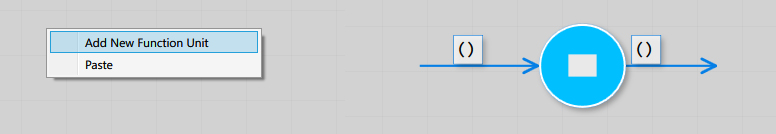
\includegraphics[width=1\linewidth]{./img/newFunctionUnit.jpg} 
			\caption{Erstellen einer neuen Funktionseinheit}
		\end{figure}
		
	
	Nach dem Erstellen einer neuen Funktionseinheit, wird diese automatisch
	selektiert und der Tastaturfokus wird in das Textfeld des Kreises gesetzt.
	Dadurch lässt sich diese benennen.
	
	Beim Klicken auf den äußeren Teil des Kreises wird die Funktionseinheit
	selektiert. Beim Klicken auf das Textfeld, wechselt der Tastaturfokus auf
	das Textfeld (ein Mouseover zeigt auch an, über welchen Teil des Kreises
	die Maus sich gerade befindet, auch ein Klicken und Ziehen um sofort ein Teil
	des Textes zu markieren bleibt damit dem Benutzer weiterhin möglich, so wie er es von
	einem Textfeld gewohnt ist).
	
			\begin{figure}[H]
				\centering
				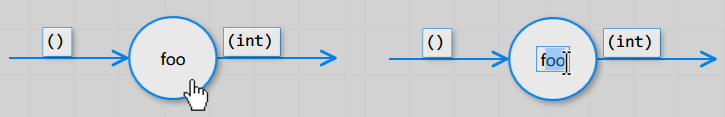
\includegraphics[width=1\linewidth]{./img/functionUnitCursor.jpg} 
				\caption{Textfeld innerhalb der Funktionseinheit}
			\end{figure}
	
	
\subsubsection{Erstellen/Löschen/Manipulieren von Inputs und Outputs}

	Eine Funktionseinheit wird standardmäßig mit einem Eingang und einem Ausgang
	erstellt. Die Daten, die aus diesen hinein- oder herausfließen, können auf
	dem Textfeld eingetragen werden. Dabei bietet diese Textfeld ein einfaches
	Syntaxhighlighting.
	
		\begin{figure}[H]
			\centering
			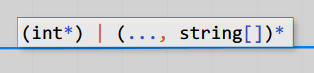
\includegraphics[width=0.4\linewidth]{./img/synatxHighlighting.jpg} 
			\caption{Syntaxhighlighting}
		\end{figure}
	
		
	Eine Funktionseinheit kann mehr als nur einen Ausgang besitzen.
	Das Hinzufügen eines neuen Ausgangs ist über \textit{Rechtsklick -> Add New Output} möglich.
	Das Löschen eines Ausgangs ist ebenso möglich.

	\begin{figure}[H]
		\centering
		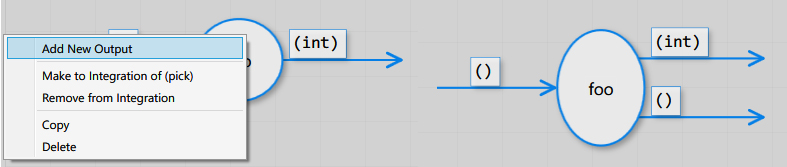
\includegraphics[width=1\linewidth]{./img/addOutput.jpg} 
		\caption{Hinzufügen eines neuen Outputs}
	\end{figure}



	Die Reihenfolge bei mehreren Ausgängen kann per Drag\&Drop verändert werden.
	
	Der Name des Ausgangs kann unterhalb des Pfeiles eingetragen werden.
	
\subsubsection{Verknüpfen und Trennen von Funktionseinheiten über Drag\&Drop }

	Wird das Ende eines Pfeiles eines Ausgangs auf eine andere Funktionseinheit gedropt, so werden beide
	miteinander Verbunden. 
	
	\begin{figure}[H]
		\centering
		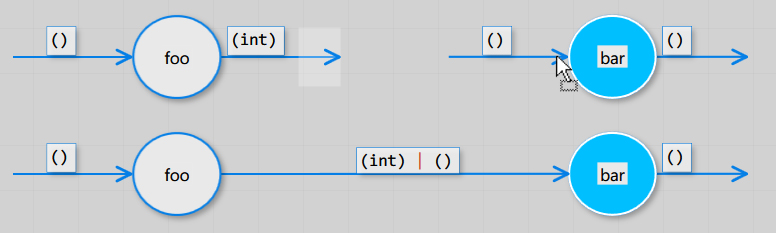
\includegraphics[width=1\linewidth]{./img/dragdrop.jpg} 
		\caption{Verbinden von Funktionseinheiten}
	\end{figure}
	
	
	
	
	Die Datennamen des Flusses werden bei nicht
	Übereinstimmung dieser mit Hilfe der Pipe-Notation in das Textfeld des nun neu
	erzeugten Datenstromes eingetragen. Stimmen beide überein, wird auf die Pipe-Notation
	verzichtet.
	
	
	
	Werden die Daten eines verbundenen Datenflusses geändert, werden die Eingänge
	und Ausgänge mit Berücksichtigung auf die Pipe-Notation angepasst, sodass
	beim Trennen der beiden Funktionseinheiten, die Änderungen erhalten bleiben.
	
	Durch Drag and Drop eines verbunden Pfeiles auf eine leere Stelle des
	Zeichenbereichs kann eine Verbindung getrennt werden. Wird sie auf eine
	andere Funktionseinheit gedropt, so wird diese als neues Ziel gesetzt und die 
	Verbindung zur vorherigen Funktionseinheit gelöscht. 
	
\subsubsection{Erstellen von Integrationen}

	Durch Rechtsklick auf eine Funktionseinheit kann im Kontextmenü der Eintrag
	\textit{Make to Integration of (Pick)} ausgewählt werden. Der Cursor verändert
	sich, wird nun eine andere Funktionseinheit angeklickt, so wird der
	komplette Flow, von der diese Funktionseinheit Teil ist, der Integration untergeordnet.
	
		\begin{figure}[H]
			\centering
			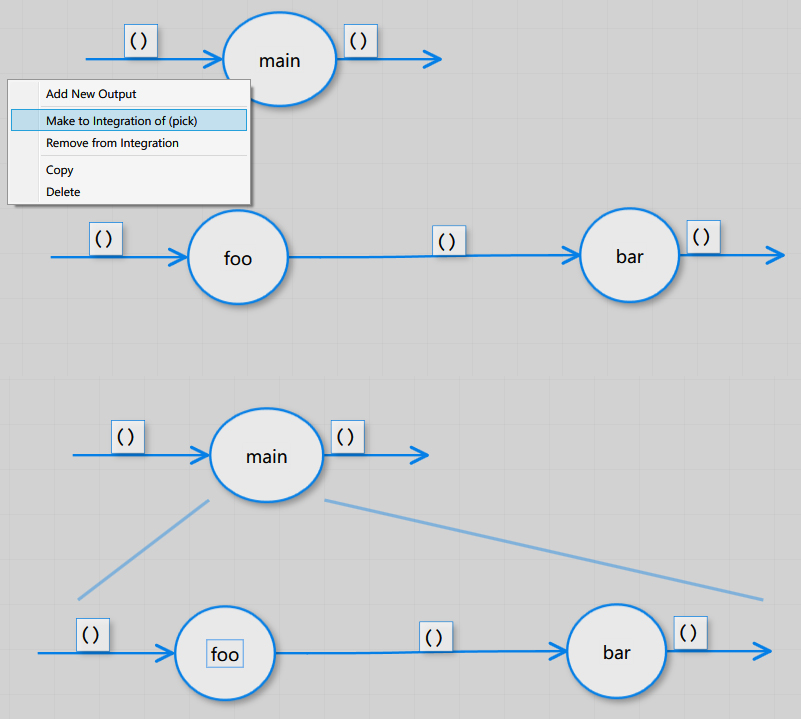
\includegraphics[width=1\linewidth]{./img/pickIntegration.jpg} 
			\caption{Erstellen von Integrationen}
		\end{figure}
		
	
	
	Das Entfernen eines Flows von einer Integration ist auch über das Kontextmenü
  möglich.
  Dabei wird der komplette zusammenhängende Flow aus der
	Integration entfernt. 
	
	
	Bei einer Modifikation des Datenflusses innerhalb einer Integration, werden nach
	bestimmten Regeln die nachfolgenden (abgetrennten) Funktionseinheiten
	ebenfalls aus der Integration entfernt. Wird die erste Funktionseinheit
	entfernt, gilt diese Regel nicht.
	
	\subsubsection{Definieren von Datentypen}

	Eigene Datentypen können auf der rechten Seite des Editors angelegt werden.
	Durch \textit{Rechtsklick -> Add New DataType}. Außerdem zeigt der obere Button an,
	ob im aktuellen Diagramm Datenflüsse mit Daten fließen, die nicht definiert
	sind (\texttt{int}, \texttt{string}, \texttt{double}, usw. werden automatisch ignoriert). Ein Klick auf diesen erstellt für jeden nicht-definierten Datentyp einen neuen Eintrag.
	Auch Datentypen innerhalb eines eigenen Datentypen werden überprüft, ob sie 
	bekannt sind oder nicht.
	
	\begin{figure}[H]
		\centering
		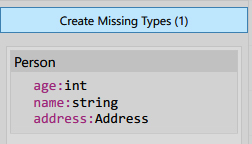
\includegraphics[width=0.4\linewidth]{./img/datatypes.jpg} 
		\caption{Der Editor überprüft, ob für \textit{Address} ein Datentyp definiert wurde.}
	\end{figure}
	
		

	
\subsubsection{Navigation und Tastenkürzel}

	Zur Navigation innerhalb des Zeichenbereichs wird das Mausrad verwendet.
	Durch Scrollen wird in den Zeichenbereich herein und heraus gezoomt.
	Durch gedrückt halten des Mausrades (mittlere Maustaste) und Bewegen der
	Maus kann die Ansicht verschoben werden (das Zeichenbereich ist endlos groß).
	
	Ein weiteres Feature besteht darin, dass ab bestimmten Zoom-Stufen die
	Schriftgrößen der Namen der Funktionseinheiten angepasst werden und die 
	Textfelder der Datenflüsse ausgeblendet werden.
	Außerdem können Textfelder nicht mehr fokussiert werden, was ein einfacheres
	Verschieben der Funktionseinheiten ermöglichen soll. Diese Gegebenheit wird
	visuell kenntlich gemacht, indem die Hintergrundfarbe des Textfeldes bei
	einer selektierten Funktionseinheit mit der Selektierungsfarbe übereinstimmt.
	Auch der Mauszeiger zeigt bei einem Mouseover an, dass nun nicht mehr in
	das Textfeld geklickt werden kann.
	
	
	\subsubsection{Weitere Features}

	\begin{itemize}
		\item Speichern, Laden, Mergen
		
		Das Speichern und Laden in drei Dateiformate wird unterstützt
		(yaml, json und xml - nach Dateigröße aufsteigend sortiert).
		Auch das Laden eines anderen Flow Designs in das aktuelle geladene wird 
		mit der Merge-Funktion unterstützt.

		\item Unhandled Exception Error Dialog
		
		Wird eine Exception geworfen, die nicht behandelt wurde, so wird eine
		allgemeine Fehlerbehandlung aufgerufen. Das Programm stürzt somit nicht ab,
		sondern ein Dialog erscheint, mit einem Stacktrace und Informationen
		über die geflogenen Exception. Der Benutzer kann entscheiden, ob er
		hier das Programm beenden, oder den Fehler ignorieren will.
		Der Stacktrace kann gegenenfalls kopiert und an den Entwickler als
		Bugreport zugeschickt werden.
		
		\item Help-Window
		
		Ein einfaches Hilfefenster, dass dem Benutzer einen Überblick über die
		vorhandenen Tastenkürzel zeigt und die Navigation mit der Maus erklärt.
	\end{itemize}
	



\subsection{Views / ViewModels}

Das Projekt wurde nicht strikt nach MVVM-Pattern (Model-View-ViewModel) 
umgesetzt, jedoch bedient es sich der Idee, das es eine View gibt, die
als Datenkontext ein ViewModel zugewiesen bekommen hat. Durch das Zuweisen eines
Datenkontextes wird es GUI-Elementen der View ermöglicht sich an Eigenschaften des ViewModels/Models zu
binden. Ein \textit{Bindung} bewirkt, dass sich das GUI-Element automatisch aktualisiert,
sobald sich die dazugehörige Eigenschaft ändert. Eine Änderung einer
Eigenschaft des ViewModels ändert somit automatisch die View.

Die GUI besteht aus mehreren Views (xaml-Dateien) und dazugehörigen ViewModels.
Die Aufgabe des ViewModels besteht vor allem darin, ein Domänenmodell entgegenzunehmen und dieses darzustellen, bzw. die aktuelle Darstellung zu aktualisieren.

Nach jeder Änderung am Domänenmodell - zum Beispiel das Hinzufügen einer neuen
Funktionseinheit -  dieses komplett neu zu laden (Löschen und neu Hinzufügen aller
ViewModels, die wiederum ein Neugenerieren der UI-Framework-Elemente zur
Folge hatte) erwies sich als nicht sehr performant. 
Ab Diagrammen, mit über 20 Nodes, stieg die Zeit zur Aktualisierung der View
bereits auf mehrere Sekunden an.
Die Lösung bestand darin, nicht einfach alles zu Löschen und neu
hinzuzufügen, sondern darin, die Änderungen am Modell zu lokalisieren und nur
diese neu zu erstellen, bzw. nur die Eigenschaften neu zu setzen. Durch
diese Verbesserungen wurde die Performance deutlich gesteigert, sodass
Diagramme mit mehreren hundert Funktionseinheiten keine spürbaren Perfomanceverluste mit
sich führen. Einzig das Duplizieren von vielen Funktionseinheiten dauert nach wie vor
etwas länger. 

\subsection{Interaktionen}

Wie bereits im Grundlagen-Teil erwähnt (Abschnitt Entwurfsmethode), schlägt Flow Design
vor, alle Events als Interaktionen zu bezeichnen und für jedes dieser
Änderungen ein eigenen Flow Design zu erstellen. 
Es bietet sich somit an, alle Interaktionen in einer Klasse zu sammeln.
Diese bietet somit einen Überblick über alle Funktionalitäten der GUI.
Da diese Integrationen sind, sind sie in der Regel leicht zu verstehen. Die
Interaktionen rufen Methoden von anderen Klassen auf, die die Operationen am
\texttt{MainModel} vereinfachen. Am Ende fast jeder Interaktion wird die \texttt{ViewRedraw} Methode aufgerufen, die das \texttt{MainViewModel} veranlasst, das Modell neu zu laden und somit die Änderungen der Interaktion in der GUI sichtbar macht.
Aus diesem Grund erwies es sich als schlecht, wenn eine Interaktion eine andere
Interaktion aufruft, um ihre Funktionalität umzusetzen. 
Stattdessen war es eine bessere Lösung, den Code der einen Interaktion in
die andere zu kopieren. Dies widerspricht zwar dem DRY Prinzip, jedoch stellt sich heraus, dass Coderedundanzen innerhalb von Integrationen nichts Schlimmes sind. Integrationen beinhalten schließlich keine Logik \footnote{Beim
Aufruf einer Funktionseinheit, die mehrere Outputs liefert, existiert
eigentlich doch Logik in der Integration (Beispiel \texttt{IsIntegration}-Methode: Wenn ja, dann X, wenn nicht, dann Y). Dadurch verlieren Integrationen etwas an ihrer
Leichtgewichtigkeit und sind nicht mehr ganz so einfach zu verstehen.} und haben eine hohe
Abstraktion.

Beispiel dieser Aussage:
\begin{lstlisting}[caption=AppendNewFunctionUnit]
public static object AppendNewFunctionUnit(FunctionUnit currentFunctionUnit, double offsetX, DataStreamDefinition outputToConnect, MainModel mainModel)
{
	var newFunctionUnit = FunctionUnitManager.CreateNew();
	
	newFunctionUnit.Position = currentFunctionUnit.Position;
	newFunctionUnit.MoveX(offsetX);
	
	// default IO of new function unit: input of new function unit = output to connect to of current function unit
	newFunctionUnit.InputStreams.Add(
		DataStreamManager.NewDefinition(newFunctionUnit, outputToConnect));
	newFunctionUnit.OutputStreams.Add(
		DataStreamManager.NewDefinition(newFunctionUnit, "()"));
	MainModelManager.ConnectTwoDefintions(outputToConnect, newFunctionUnit.InputStreams.First(), mainModel);
	
	mainModel.FunctionUnits.Add(newFunctionUnit);
	
	ViewRedraw();
	
	return newFunctionUnit;
}
\end{lstlisting}

\begin{lstlisting}[caption=CreateNewOrGetFirstIntegrated]
public static FunctionUnit CreateNewOrGetFirstIntegrated(FunctionUnit currentFunctionUnit, MainModel mainModel)
{
	FunctionUnit @return = null;
	
	currentFunctionUnit.IsIntegration(
		isIntegration: () => @return = 		currentFunctionUnit.IsIntegrating.First(),
		isNotIntegration: () =>
		{
			var newFunctionUnit = FunctionUnitManager.CreateNew();
			newFunctionUnit.Position = currentFunctionUnit.Position;
			newFunctionUnit.MoveY(100);
			
			newFunctionUnit.InputStreams.Add(
			DataStreamManager.NewDefinition(newFunctionUnit, currentFunctionUnit.InputStreams.First()));
			newFunctionUnit.OutputStreams.Add(
			DataStreamManager.NewDefinition(newFunctionUnit, "()"));
			
			currentFunctionUnit.IsIntegrating.Add(newFunctionUnit);
			
			mainModel.FunctionUnits.Add(newFunctionUnit);
			
			@return = newFunctionUnit;
			ViewRedraw();
		});
	
	return @return;
}
	\end{lstlisting}





	Die \texttt{AppendNewCell}-Methode erzeugt eine neue Funktionseinheit und 
	verschiebt diese entlang der X-Postion.
	Außerdem setzt sie den Input gleich der \texttt{DataStreamDefinition} die
	übergebenen wurde und verbindet diese beide.
	\texttt{AppendNewCell} wird durch die Tastenkombination Ctrl-Tab ausgelöst, wenn
	sich der Tastaturfokus innerhalb eines Textfeldes einer View einer Funktionseinheit, oder eines Ausgangs befindet. Bei dem ersten Fall wird der erste unverbundene Ausgang genommen, an dem die neue Funktionseinheit angehängt wird \footnote{nicht Teil der gezeigten Methode.} .
	
	Beide Methoden geben eine
	Domänenmodell-Instanz als \texttt{object} an die GUI zurück. Die GUI-Logik findet dann die
	dazugehörige View und setzt den Fokus auf diese.
	
	Beide Methoden sind Methoden aus der Interaktions-Klasse, sie werden also
	direkt aus einem Event von der GUI ausgelöst. 
	Beide Methoden haben ähnliche Methodenaufrufe (Neue Funktionseinheit
	erzeugen, sie auf die gleiche Position zu setzten wie die der übergebenen
	Funktionseinheit, neue Standardwerte für den Output-Stream der neuen
	Funktionseinheit setzen, dem \texttt{MainModel} die neue Funktionseinheit hinzufügen
  und die Ansicht neu zu zeichnen).
  Diese könnten in eine neue Integration ausgelagert werden, hätte jedoch eine unnötige
	Verschachtlung von Code als Auswirkung. Besser ist es hier die
	Coderedundanzen nicht als Code-Smell zu sehen und diese zu belassen.
	So ist auf einen Blick ersichtlich, was die Interaktion genau macht, ohne
	im Code herum springen zu müssen.






\subsection{Validierung des Datenflusses - Farbliche Kennzeichnung }

Eine Instanz vom Typ ValidationException kann dem ViewModel übergeben werden.
Die ValidationException beinhaltet die Information, ob es sich um eine Fehler oder um eine Warnung handelt (Fehler werden rot markiert, Warnungen grün), welche Elemente den Fehler anzeigen sollen, sowie einen Fehlertext, der als Tooltip an dem Element angezeigt wird.

\begin{figure}[H]
	\centering
	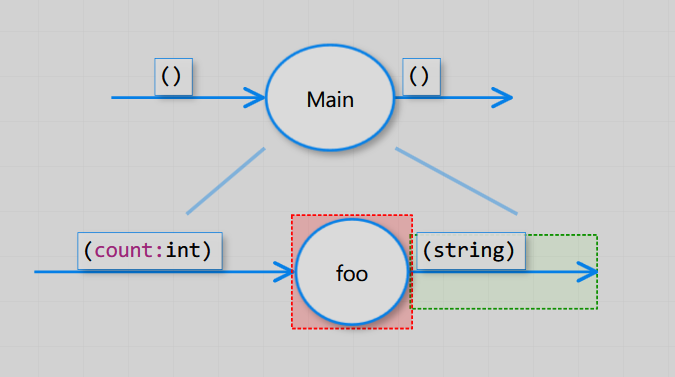
\includegraphics[width=0.6\linewidth]{./img/DexelValidation.png}
	\caption{Dexel - Warnung- und Fehler-Darstellung}
\end{figure}



\section{Roslyn - Generierung von Code aus einem Diagramm}

Da eine Flow Design auf unterschiedlichen Weisen im Code umgesetzt werden
kann, mussten hier Entscheidungen getroffen werden, in welchen Fällen
welche Weise gewählt wird. Wird das Projekt fortgeführt, könnte man in
Betracht ziehen, dem Nutzer einige Optionen zur Konfiguration der Generierung
zur Verfügung zu stellen. Aktuell bietet das Programm nur die hier vorgestellte Weise zur Verfügung.


\subsection{Vorstellung - was erreicht wurde}

Um den aktuellen Stand der Code-Generierung zu präsentieren, werden nachfolgend zwei Beispiele 
vorgestellt.

\subsubsection{CSV Tabellieren -  Beispiel aus YouTube Video von Ralf Westphal und Stefan Lieser}

Die Aufgabe besteht darin, den Inhalt einer CSV-Datei in eine ACSII-Tabelle zu formatieren \cite[S.12]{kata}.
\begin{figure}[H]
	\centering
	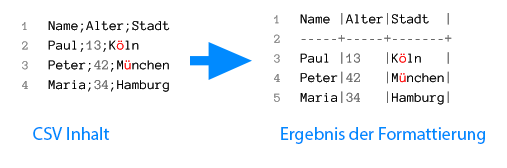
\includegraphics[width=0.8\linewidth]{./img/csvAufgabe.png}
	\caption{Aufgabe - CSV Tabellieren}
\end{figure}


Das Flow Design, das Ralf Westphal und Stefan Lieser in dem Video entwerfen sieht folgendermaßen aus. \footnote{Video CSV Tabellarisieren \cite{youtubevideos}}


\begin{figure}[H]
	\centering
	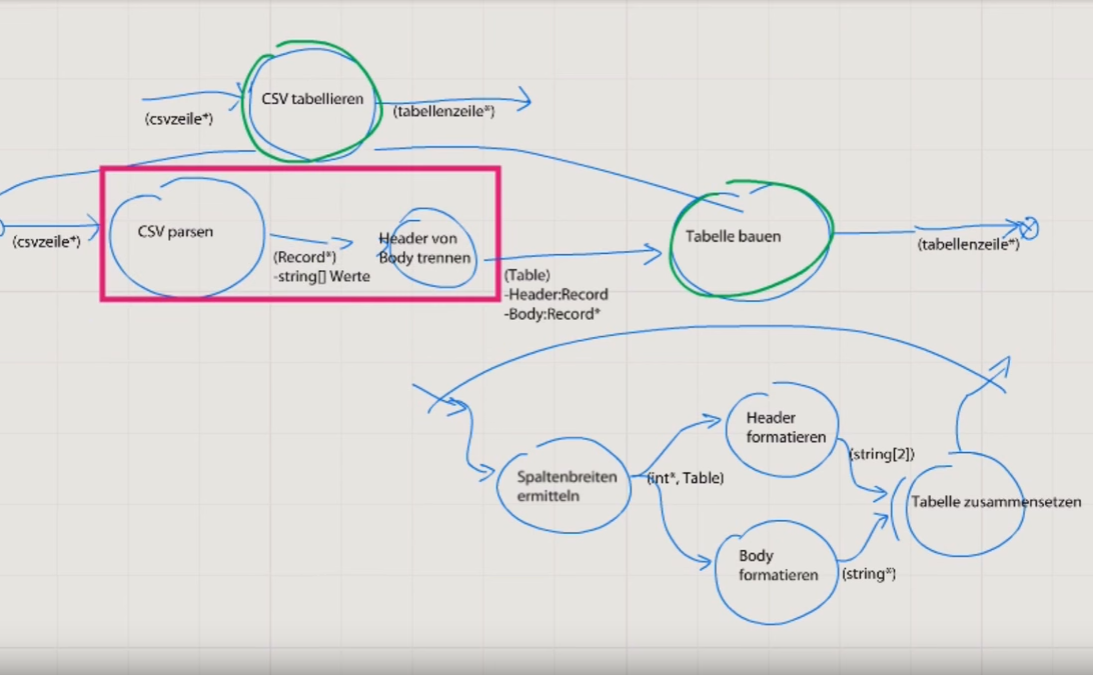
\includegraphics[width=1\linewidth]{./img/youtubeflowdesign.png}
	\caption{CSV Tabellarisieren - Flow Design aus YouTube Video}
\end{figure}


Nun das Flow Design umgesetzt in Dexel. Zu beachten ist, das die Split Output und Joined Input Notation mit der Pipe-Notation ersetzt wurde, da Dexel aktuell keine Joined-Notation unterstützt.


\begin{figure}[H]
	\centering
	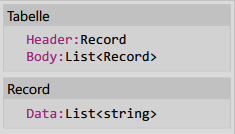
\includegraphics[width=0.4\linewidth]{./img/csvtabellierenDexelDataTypes.png}
	\caption{CSV Tabellarisieren - Datentypen}
\end{figure}




\begin{landscape}
\begin{figure}
	\thispagestyle{empty}
	    \makebox[\linewidth]{
	    		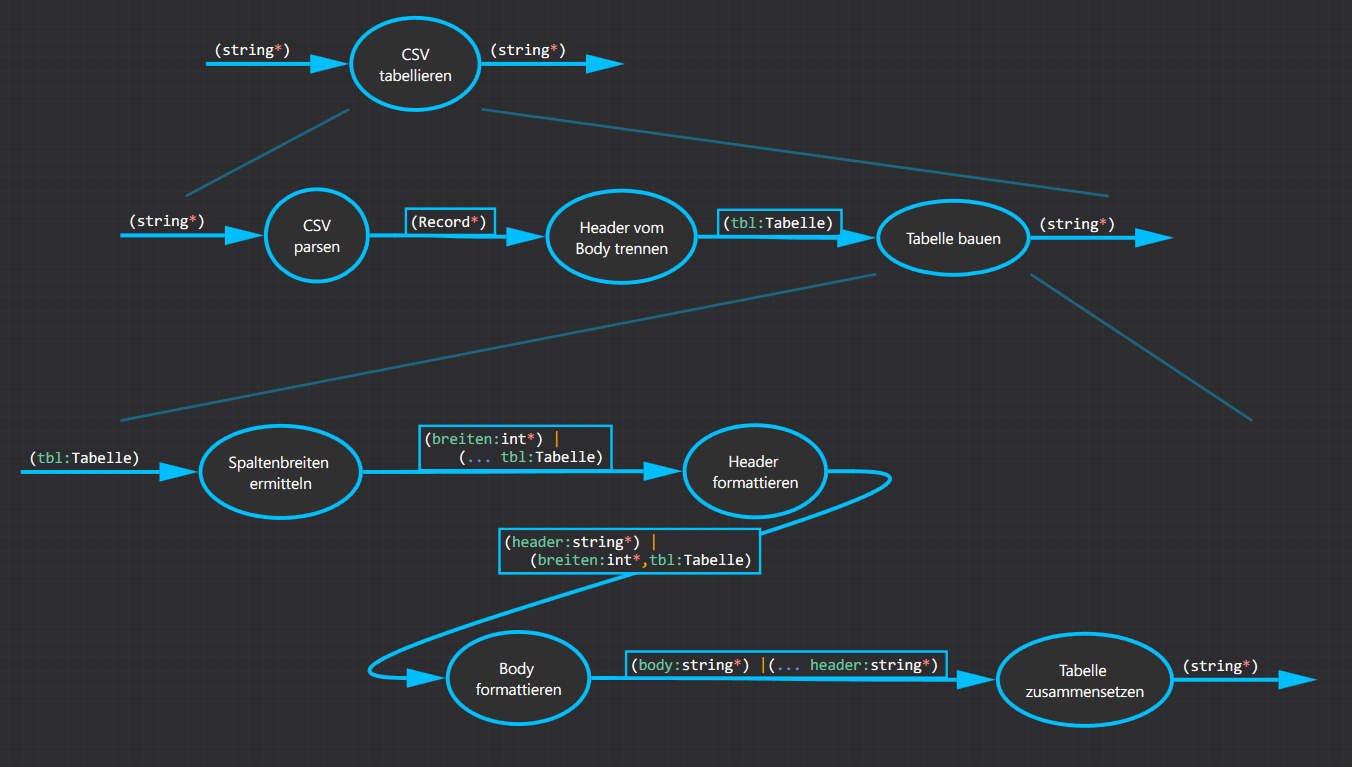
\includegraphics[width=1.1\linewidth]{./img/csvtabellierenDexel.png}
	    }

	\caption{CSV Tabellarisieren - Dexel Flow Design}
\end{figure}
\end{landscape}






\begin{lstlisting} [caption = CSV tabellieren mit Dexel generierter Code]
// Integrationen
public static IEnumerable<string> CSVTabellieren( IEnumerable<string> strings)
{
	var records = CSVParsen(strings);
	var tbl = HeaderVomBodyTrennen(records);
	return TabelleBauen(tbl);
}

public static IEnumerable<string> TabelleBauen(Tabelle tbl)
{
	var breiten = SpaltenbreitenErmitteln(tbl);
	var header = HeaderFormattieren(breiten, tbl);
	var body = BodyFormattieren(breiten, tbl);
	return TabelleZusammensetzen(body, header);
}
\end{lstlisting}

\begin{lstlisting} [caption = CSV tabellieren mit Dexel generierter Code]
// Datentypen
public class Tabelle
{
	public Record Header;
	public List<Record> Body;
}

public class Record
{
	public List<string> Data;
}
\end{lstlisting}

\begin{lstlisting} [caption = CSV tabellieren mit Dexel generierter Code]
// Operationen
public static IEnumerable<int> SpaltenbreitenErmitteln(Tabelle tbl)
{
    throw new NotImplementedException();
}

public static IEnumerable<string> HeaderFormattieren(IEnumerable<int> breiten, Tabelle tbl)
{
    throw new NotImplementedException();
}

public static IEnumerable<string> BodyFormattieren(IEnumerable<int> breiten, Tabelle tbl)
{
    throw new NotImplementedException();
}

public static IEnumerable<string> TabelleZusammensetzen(IEnumerable<string> body, IEnumerable<string> header)
{
    throw new NotImplementedException();
}

public static Tabelle HeaderVomBodyTrennen(IEnumerable<Record> records)
{
    throw new NotImplementedException();
}

public static IEnumerable<Record> CSVParsen(IEnumerable<string> strings)
{
    throw new NotImplementedException();
}
\end{lstlisting}

Der Datenfluss in den beiden Integrationen wurde korrekt generiert. 
Außerdem wurden alle Datentypen und Methodensignaturen der Operationen erzeugt.

\pagebreak

\subsubsection{Shopping Simulator - Komplexeres Beispiel}

Dieses Beispiel soll zeigen, wie auch mehreren Ausgänge von Funktionseinheiten und Streams korrekt generiert werden.

Der Methode \texttt{ShoppingSimulator} wird eine Anzahl an Kunden übergeben, die generiert werden soll.
Jeder Kunde ist eine Person, die noch zusätzlich zu Name und Alter ein Budget hat.
Diese drei Eigenschaften werden für jeden Kunde zufällig generiert.
Anschließend wird ein zufälliger Einkaufswagen erzeugt und die beiden Objekte (Einkaufswagen und Kunde) durchlaufen eine \texttt{Checkout}-Routine.
Das Ergebnis wird in die Konsole ausgegeben.

Eine mögliche Konsolenausgabe - nachdem die Methodenrümpfe der Operationen von Hand implementiert wurden - wäre:
\begin{figure}[H]
	\centering
	\includegraphics[width=0.6\linewidth]{./img/ShoppingSimulator_result.png}
	\caption{Konsolenausgabe - ShoppingSimulator}
\end{figure}



\begin{landscape}
	\begin{figure}
		\thispagestyle{empty}
		\vspace*{-1.5cm}
		\makebox[\linewidth]{
			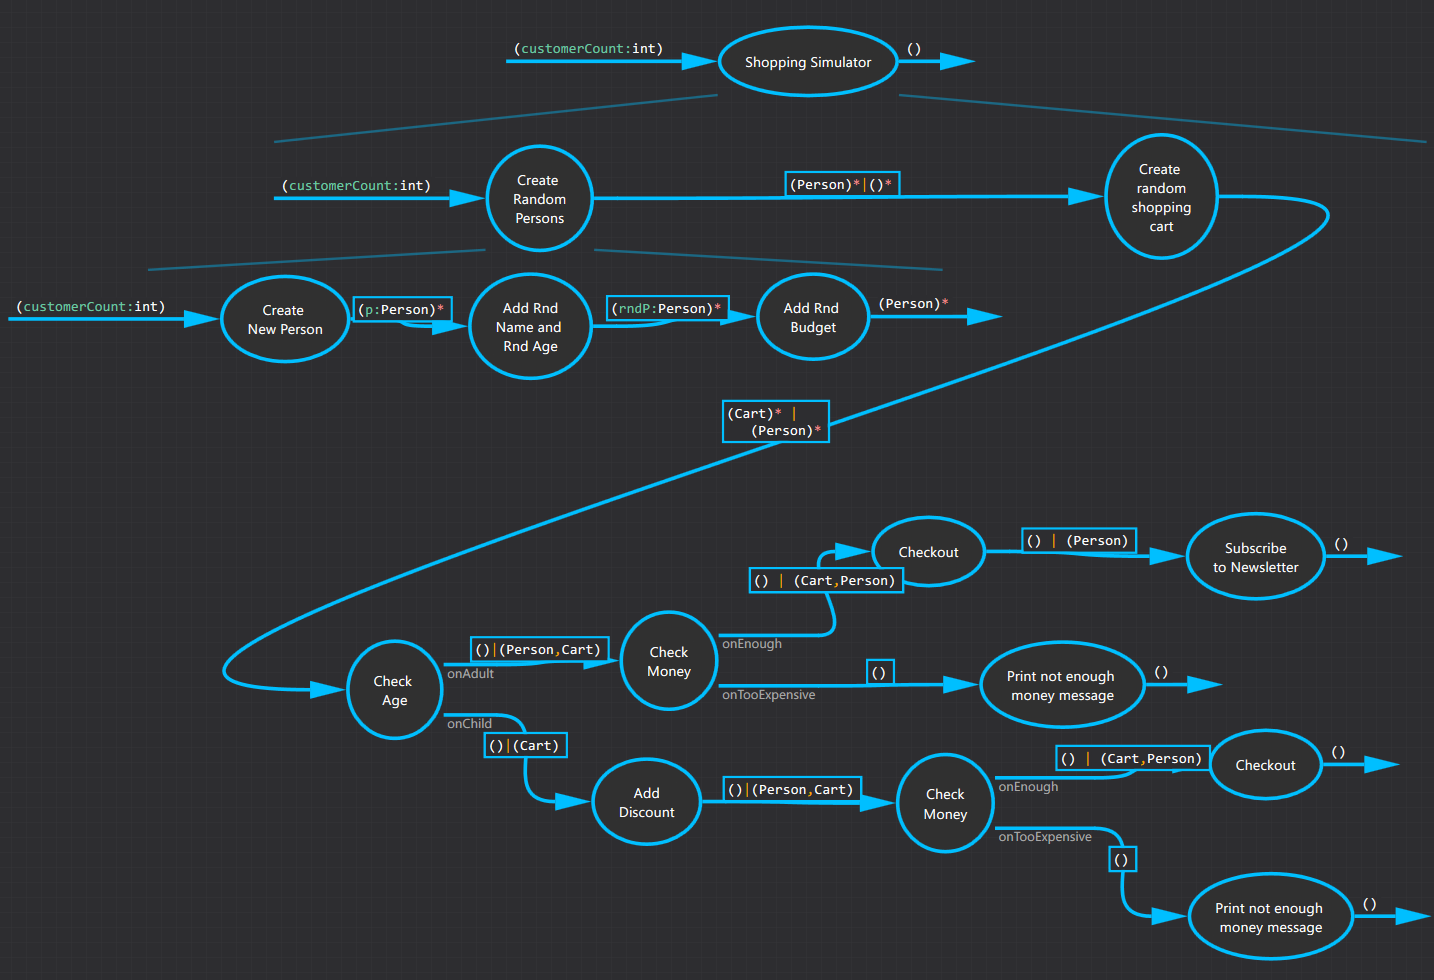
\includegraphics[width=1.15\linewidth]{./img/shoppingSimulator.png}
		}
		
		\caption{Shopping Simulator}
	\end{figure}
\end{landscape}




\begin{lstlisting}[caption=Shopping Simulator - automatisch generierter Code mit Dexel]
// Integration
public static void ShoppingSimulator(int customerCount)
{
	CreateRandomPersons(customerCount, person => {
		var aCart = CreateRandomShoppingCart();
		CheckAge(person, onAdult: () => {
			CheckMoney(person, aCart, onEnough: () => {
				Checkout(aCart, person);
				SubscribeToNewsletter(person);
			}, onTooExpensive: () => {
				PrintNotEnoughMoneyMessage();
			});
		}, onChild: () => {
			AddDiscount(aCart);
			CheckMoney(person, aCart, onEnough: () => {
				Checkout(aCart, person);
			}, onTooExpensive: () => {
				PrintNotEnoughMoneyMessage();
			});
		});
	});
}
\end{lstlisting}

\begin{lstlisting}[caption=Shopping Simulator - automatisch generierter Code mit Dexel]
// Datentypen
public class Person
{
	public int Age;
	public string Name;
	public double Budget;
}

public class Cart
{
	public List<string> Products;
	public double Discount;
	public double PriceTotal;
}
\end{lstlisting}


\begin{lstlisting}[caption=Shopping Simulator - automatisch generierter Code mit Dexel]
// Operationen
public static void CreateRandomPersons(int customerCount, Action<Person> onPerson)
{
	CreateNewPerson(customerCount, p => {
		var rndP = AddRndNameAndRndAge(p);
		onPerson(AddRndBudget(rndP));
	});
}

public static Cart CreateRandomShoppingCart()
{
    throw new NotImplementedException();
}

public static void CheckAge(Person aPerson, Action onAdult, Action onChild)
{
    throw new NotImplementedException();
}

public static void CheckMoney(Person aPerson, Cart aCart, Action onEnough, Action onTooExpensive)
{
    throw new NotImplementedException();
}

public static void AddDiscount(Cart aCart)
{
    throw new NotImplementedException();
}

public static void SubscribeToNewsletter(Person aPerson)
{
    throw new NotImplementedException();
}

public static void PrintNotEnoughMoneyMessage()
{
    throw new NotImplementedException();
}

public static void Checkout(Cart aCart, Person aPerson)
{
    throw new NotImplementedException();
}

public static void CreateNewPerson(int customerCount, Action<Person> onP)
{
    throw new NotImplementedException();
}

public static Person AddRndNameAndRndAge(Person p)
{
    throw new NotImplementedException();
}

public static Person AddRndBudget(Person rndP)
{
    throw new NotImplementedException();
}


\end{lstlisting}

\subsubsection{Aktueller Stand}

Die weniger komplexeren Aufgaben wurden vollständig implementiert.
Diese wären: 
\begin{itemize}
	\item Generierung der benutzerdefinierten Datentypen, und 
	\item Generierung der Methodensignaturen einer Funktionseinheit.
\end{itemize}

Die Generierung der Methodenrümpfe von Integrationen wurde auch zum Großteil implementiert.
Jedoch kann erst durch ein prototypischen Einsatz herausgefunden werden, in welchen Fällen ein Flow-Design-Diagramme noch fehlerhaft interpretiert wird. Dafür fehlt im Rahmen dieser Arbeit aber die Zeit.

Die Validierung des Datenflusses ist eng an die Generierung gekoppelt, deswegen gilt das selbe auch für diese. 

Auch bei der Generierung von Namen wird aktuell noch nicht in jedem Fall überprüft, ob es zu einer Überschneidung kommt und ob gegebenenfalls der Name angepasst werden muss.

\bigskip

Um Code zu generieren muss im Editor in der Menüleiste der Eintrag Output angesteuert werden.
Hier gibt es die Möglichkeit das aktuelle Flow Design in eine Datei auf den Desktop zu
generieren, den Code in die Konsole auszugeben, oder den Code direkt in die Zwischenablage zu kopieren (um den erzeugten Code bequem an eine gewünschte Stelle eingefügt werden kann).

Außerdem gibt es die Option eine automatische Generierung einzuschalten, die
den Code während der Bearbeitung immer neu generiert und in die Datei
auf den Desktop schreibt. So lässt sich das Ergebnis der Generierung während der Bearbeitung
des Datenflusses beobachten (vor allem in Kombination mit einem
Texteditor, wie zum Beispiel Atom, die bei einer Änderung der Datei diese automatische neu laden).

Das Ergebnis wird auch immer mit in die Konsole ausgegeben, die beim
Programmstart mit geöffnet wird.


\subsection{Kleiner Einblick in die API von Roslyn}

Das Projekt Rosyln von Microsoft ist ein .NET-Compiler, der eine API bietet, um beliebigen C\#- und und VB.NET-Quelltext zu erstellten,
zu analysieren und zu modifizieren.

Das hier verwendetet Nuget-Paket ist: Microsoft.CodeAnalysis

Der Datentypen auf dem die Methoden zum Erstellen von Code arbeitet lautet:
\texttt{SyntaxNode} 

Diese \texttt{SyntaxNodes} werden von einem Syntaxgenerator erstellt.
Dieser muss beim Initialisieren konfiguriert werden.

\begin{lstlisting}[caption=SyntaxGenerator für C\# erhalten]
var workspace = new AdhocWorkspace();
// Get the SyntaxGenerator for the specified language
var generator = SyntaxGenerator.GetGenerator(workspace, LanguageNames.CSharp);
\end{lstlisting}


Das Erstellen eines Ausdruckes, Klasse oder Methode mit Hilfe von Methoden
des Syntaxgenerators liefern am Ende immer eine \texttt{SyntaxNode} zurück.
Beim Erstellen einer Methode oder Klasse kann der Inhalt des Scopes durch
ein Array von \texttt{SyntaxNodes} bestimmt werden.

Nachfolgend ein einfaches Beispiel zum Erstellen von einem
benutzerdefinierten Datentyp.

\begin{figure}[H]
	\centering
	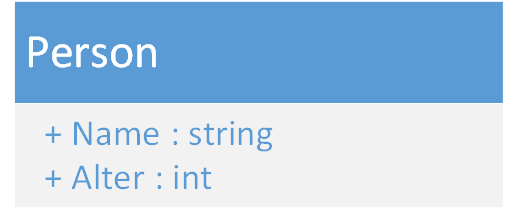
\includegraphics[width=0.3\linewidth]{./img/Person.png}
	\caption{Datentyp der generiert werden soll}
\end{figure}

	\subsubsection{Erzeugung eines Datentypen als einfaches Beispiel}
	
	\begin{lstlisting}[caption=Erzeugung einer Person-Klasse mit Roslyn]
SyntaxNode fieldName = generator.FieldDeclaration(
	name: "Name",
	type: generator.TypeExpression( SpecialType.System_String),
	accessibility: Accessibility.Public);

SyntaxNode fieldAlter = generator.FieldDeclaration(
	name: "Alter",
	type: generator.TypeExpression( SpecialType.System_Int32),
	accessibility: Accessibility.Public);

SyntaxNode[] allFields =  new[] {fieldName, fieldAlter};


// Generate the class
SyntaxNode classDefinition = Generator.ClassDeclaration(
	"Person", 
	typeParameters: null,
	accessibility: Accessibility.Public,
	modifiers: DeclarationModifiers.None,
	baseType: null,
	interfaceTypes: null,
	members:allFields
);
	\end{lstlisting}
	
	Um am Ende den Code in Form eines Strings zu erhalten muss auf die oberste
	\texttt{SyntaxNode} folgende beide Methoden aufgerufen werden:
	
	\begin{lstlisting}[caption=Erhalten des Codes als string]
	string code = classDefinition.NormalizeWhitespace().ToFullString();
	\end{lstlisting}


\subsection{Erzeugung von Methodensignaturen}

Das Analysieren einzelner Funktionseinheiten anhand ihrer Ein- und Ausgänge erlaubt eine automatische Generierung der Methodensignaturen.
Dieses Feature wurde vollständig implementiert, da die möglichen Faktoren, die Einfluss auf die Methodensignatur haben überschaubar sind und somit alle Kombinationen sich schnell herauskristallisiert haben.

\subsubsection{Output über Rückgabewert}

	Der einfachste Fall ist eine Funktionseinheit, die nur ein Ausgang hat und
	dieser auch kein Stream und auch nicht optional ist.\footnote{Im Editor ist das vorhanden sein eines Eingangs vorgeben und es gibt auch keine Möglichkeit einen weiteren Eingangs-Datenstrom zu einer Funktionseinheit hinzuzufügen. Nur Ausgänge lassen sich hinzufügen und entfernen.}
	
	In diesem Fall werden die ausgehenden Daten einfach als Rückgabewert heraus gereicht.
	
	
	\begin{figure}[H]
		\centering
			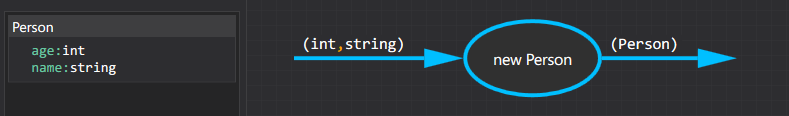
\includegraphics[width=\linewidth]{./img/roslyn_simpleOutput.png} 
		\caption{Dexel-Screenshot: Einfache Funktionseinheit mit benutzerdefinierten Datentyp}
	\end{figure}

	
	Die Generierung erzeugt folgenden Code:
	\begin{lstlisting}[caption=Mit Dexel generierter Code ]
public class Person
{
	public string Name;
	public int Age;
}

public static Person NewPerson(int aint, string astring)
{
	throw new NotImplementedException();
}
	\end{lstlisting}
	
	Hat ein Output mehr als ein Datentyp, ist kein Stream und ist auch nicht optional, so
	wird das Ergebnis als Tupel über den Rückgabewert geliefert.
	
		\begin{figure}[H]
			\centering
			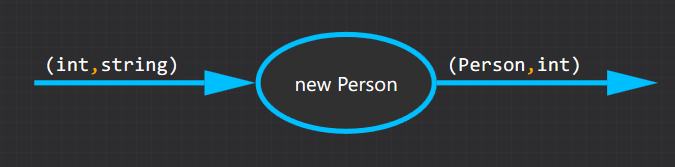
\includegraphics[width=.8\linewidth]{./img/roslyn_twoDatatypesOneOutput.png} 
			\caption{Dexel-Screenshot: Funktionseinheit mit Tupel-Output}
		\end{figure}

	
	
	\begin{lstlisting}[caption=Mit Dexel generierter Code ]
public static Tupel<Person, int> NewPerson(int aInt, string aString)
{
	throw new NotImplementedException();
}
	\end{lstlisting}

	
\subsubsection{Outputs über Actions}

	 Durch die optionale Vergabe eines Namens für den Ausgang (\textit{Actionname})  steuert der Anwender indirekt, ob ein Ausgang durch eine Action realisiert werden soll\footnote{Diese Regel wurde im Rahmen dieser Anwendung so festgelegt.}. 
	
	Ausgänge müssen nicht zwingend mit
	der Anzahl an Aufrufe der Funktionseinheit übereinstimmen. Ein Action muss
	nicht aufgerufen werden, oder kann bei einem einzigen Aufruf der Funktionseinheit auch
	mehrmals aufgerufen werden (der Beginn eines Streams). 
	
	Sobald auch eine Funktionseinheit mehrere Ausgänge hat, diese jedoch nicht
	optional sind, werden diese jedoch trotzdem als Actions realisiert, selbst wenn sie kein
	Actionname zugeordnet bekommen haben. Der Name des Actions wird dann
	automatisch generiert\footnote{	Durch Analyse der Datentypen. Ein \textit{(Person)} wird zu einem \texttt{onPerson}. Ein \textit{()} wird zu einem \texttt{continueWith}.}.
	
	Durch diese Entscheidungen gibt es keine invaliden Kombinationen an
	Ausgängen einer Funktionseinheit.
	
	
	Werden alle Ausgänge mit Actions realisiert, entfällt der Rückgabewert in diesem Fall komplett.
	
	Die Input-Daten werden in der Signatur zuerst aufgelistet, anschließend die Actions.
	
			\begin{figure}[H]
				\centering
				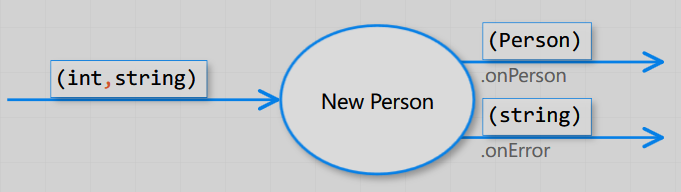
\includegraphics[width=\linewidth]{./img/roslyn_multipleOutputs.png} 
				\caption{Dexel-Screenshot: Funktionseinheit mit zwei Outputs mit definierten Actionnamen}
			\end{figure}
			
	

	
	\begin{lstlisting}[caption=Mit Dexel generierter Code ]
	public static void NewPerson(int aint, string astring, Action<Person> onPerson, Action<string> onError)
	{
	throw  new NotImplementedException();
	}
	\end{lstlisting}
	 \subsubsection{Streams}

	Streams werden in Dexel ebenfalls mit Actions realisiert, mit einer Ausnahme:
	
	Sind ist sowohl der Eingang als auch der Ausgang ein Stream und ist der \textit{Actionname} dieses Ausgangs \textit{nicht} angegeben, so wird  implizit davon ausgegangen, dass für jeden Aufruf der Funktionseinheit dieser Ausgang erzeugt wird. 
	
	Somit kann für diesen Ausgang auf eine Action verzichtet werden und der Rückgabewert genutzt werden, was eine einfachere Verwendung dieser Funktionseinheit im Code zur Folge hat.
	\footnote{	Das Vorhandensein von einem Inputstream und einem Outputstream bedeutet eigentlich nicht zwingend , dass für jeden Input auch ein Output erzeugt wird. Die Notation unterscheidet beide Fälle nicht. Deswegen die Lösung über eine Vergabe eines \textit{Actionnamen} als Kompromiss zu sehen, wodurch dem Benutzer hier eine Kontrolle über die Erzeugung des Codes geben wird. Wenn der Benutzer ein \textit{Actionname} angibt, wird indirekt davon ausgegangen, dass der Benutzer den Output auch als Action umsetzten möchte und die Funktionseinheit somit beliebig oft diese Action aufrufen kann. Ob dieses Entscheidung richtig war müsste  noch in der Praxis erprobt werden. Stellt sich heraus,	dass sie schlecht ist, müsste man über eine Anpassung der Notation nachdenken.}
	
	\begin{figure}[H]
		\centering
		\includegraphics[width=.9\linewidth]{./img/roslyn_Stream.png} 
		\caption{Dexel-Screenshot: Funktionseinheit mit Stream als Ausgang}
	\end{figure}
	


	
	
\begin{lstlisting}[caption=Mit Dexel generierter Code ]
public static void NewPersons(int aInt, string aString, Action<Person> onPerson)
{
	throw new NotImplementedException();
}
\end{lstlisting}
	
		
	\begin{figure}[H]
		\centering
		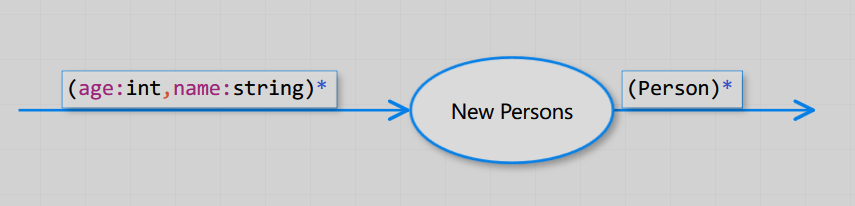
\includegraphics[width=.9\linewidth]{./img/roslyn_StreamStream.png} 
		\caption{Dexel-Screenshot: Funktionseinheit mit eingehendem und ausgehendem Stream und undefinierten Actionnamen}
	\end{figure}
			

	\begin{lstlisting}[caption=Mit Dexel generierter Code ]
public static Person NewPersons(int age, string name)
{
	throw new NotImplementedException();
}
	\end{lstlisting}
	 

\subsection{Erzeugung des Methodenrumpfes einer Integration}
\label{sec:orgheadline51}


	 \subsubsection{Terminologie}

	Eine Integration kann nicht nur aus
	Operationen bestehen, sondern auch aus anderen Integrationen bestehen.
	Leider gibt es hierfür keine Überbegriff für beide.
	Da im in diese Kapitel jedoch öfters von Funktionseinheiten innerhalb einer
	Integration die Rede sein wird, muss hierfür ein Überbegriff eingeführt
	werden. Funktionseinheiten, die sich in einer Integration befinden, werden
	nachfolgend als Sub-Funktionseinheiten bezeichnet.
	
	\subsubsection{Die Herangehensweise}

	
	Die automatische Erzeugung einer Integration ist die komplexeste Aufgabe in
	diesem Projekt. Um die Aufgabe überschaubar zu halten, wurde diese im Groben in
	zwei Teileaufgaben zerteilt: die Analyse und die Generierung.
	Die Analyse besteht wiederum aus unterschiedlichen Methoden, die jeweils das
	Flow Design auf eine bestimme Sache analysieren und das Ergebnis in ein Objekt
	abspeichern. Diese Objekt wurde als \texttt{IntegrationBody} bezeichnet.
	Diese beinhaltet alle Informationen aus der Analyse. Am Ende wird dieses Objekt
	der Generierungsmethode übergeben, die anhand diesem den Code erzeugt\footnote{Ein weiterer Vorteil dieser Aufteilung ist, dass ein großer Teil frei von der Roslyn-API bleibt. Die eigenen Datentypen lassen sich dazu auch besser testen, als die SyntaxNodes von Roslyn. Möchte man das Ergebnis von Roslyn testen, bleibt einem  oft keine andere Wahl, als den erzeugten Code samt Whitespaces über ein String-Vergleich zu erschlagen, was bei mehrzeiligem Code doch etwas ausufern kann. Stattdessen lässt sich das Ergebnis aus den eigenen Analysen hingegen einfach über ein Vergleich von den gefundenen Objekt-Referenzen überprüfen.}.
	
\begin{landscape}
	\begin{figure}
		\thispagestyle{empty}
		\vspace*{-1.5cm}
		\hspace*{-0cm}
		\makebox[\linewidth]{
			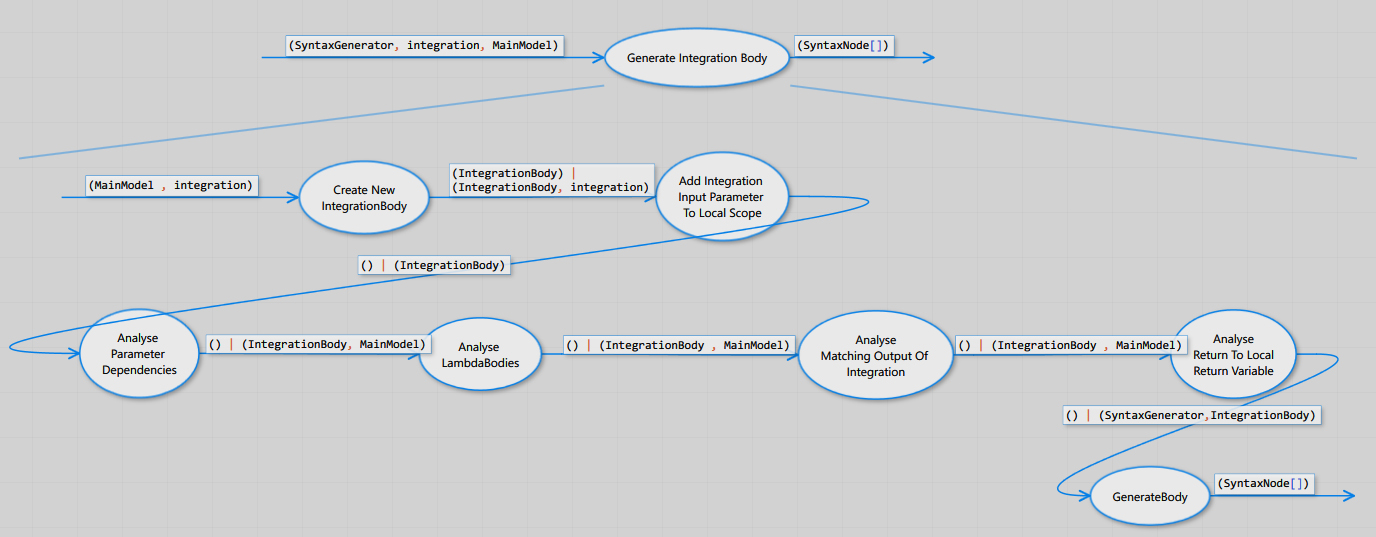
\includegraphics[width=1.15\linewidth]{./img/GenerateIntegrationBody.jpg}
		}
		
		\caption{Generate Integration Body - Flow Design}
	\end{figure}
\end{landscape}
	
	\subsubsection{Analyse des Flow Designs}

	\begin{enumerate}
		\item \texttt{AnalyseParameterDependencies}

		Da die Pipe-Notation unterstützt wird, reicht es nicht einfache aus die Daten
		aus den Datenflüssen zu nehmen, die direkt in die aktuelle
		Funktionseinheit fließen. Stattdessen muss der Fluss rückwärts
		traversiert werden und auf Übereinstimmungen untersucht werden.
		Für jede Sub-Funktionseinheit muss diese Analyse durchgeführt werden.
		Für jeden Input-Datentyp jeder Funkionseinheit wird das Ergebnis gespeichert.
		Das Ergebnis beinhaltet ob der Datentyp gefunden
		wurde, ob er im Eingang der Integration gefunden wurde, oder ob er aus einer
		anderen Sub-Funktionseinheit innerhalb des Datenflusses stammt. 
		Ein Aufruf einer Sub-Funktionseinheit kann nur generiert werden, wenn alle Datentypen gefunden
		wurden.
		
		\item \texttt{AnalyseLambdaBodies}

		Manche optionale Datenflüsse oder Stream werden über Actions realisiert.
		Das bedeutet, dass sich alle nachfolgenden Funktionseinheiten innerhalb
		des Lambda-Ausdruckes befinden müssen. Die Analyse speichert das Ergebnis
		in folgender Form ab. 
		
		\begin{lstlisting}[caption=LambdaBody Klasse]
public class LambdaBody
{
	public DataStreamDefinition InsideLambdaOf;
	public FunctionUnit FunctionUnit;
}
		\end{lstlisting}
		
		Da die \texttt{LambdaBody}-Objekte in der Reihenfolge im \texttt{IntegrationBody} abgelegt
		werden, in der sie im Flow Design vorkommen, kann daraus auch später die
		Reihenfolge der zu generierenden Methoden abgeleitet werden.
		
		
		Für jede Funktionseinheit wird solch ein Objekt angelegt, auch wenn es
		nicht innerhalb eines Lambda-Ausdrucks vorkommt. Ist das der Fall, so ist der Wert
		\texttt{InsideLambdaOf} \texttt{null} . Alle Funktionseinheiten für die dieser Wert
		\texttt{null} ist, befinden sich somit direkt im Scope der Integration und nicht
		innerhalb eines Lambda-Ausdrucks.
		
		\item \texttt{AnalyseMatchingOutputOfIntegration}

		Hat die Integration einen Ausgang der als Action realisiert werden muss, so
		muss herausgefunden werden, welche Sub-Funktionseinheiten diesen
		Ausgang bedienen. Dabei werden die Implementierungs-Stile der
		beiden übereinstimmenden Ausgänge mit abgespeichert. Später bei der
		Generierung gibt es somit vier Möglichkeiten:
		\begin{itemize}
			\item Beide sind Actions
			
			Die Action der Integration wird direkt an die Sub-Funktionseinheit
			weitergereicht. Dadurch erlaubt man einer Sub-Funktionseinheit das
			Aufrufen des Ausgang der Integration.
			
			\begin{lstlisting}[caption=Action-Action-Beziehung]
// Integration
public static void Main(Action<string> onError)
{
	DoSomething(onError);
}

// Operation
public static void DoSomething(Action<string> onError)
{
	throw new NotImplementedException();
}
			\end{lstlisting}
			
			
			\item Integrationsausgang ist Action, Sub-Funktionseinheitsausgang ist
			Rückgabewert 
			
			Die Action wird aufgerufen mit dem Methodenaufruf als Parameter.
			
\begin{lstlisting}[caption=Action-Return-Beziehung]
public static void CreateRandomPersons(int customerCount, Action<Person> onPerson)
{
	CreateNewPerson(customerCount, p => {
		var rndP = AddRndNameAndRndAge(p);
		onPerson(AddRndBudget(rndP));
	});
}
\end{lstlisting}
			\item Integrationsausgang ist Rückgabewert, Sub-Funktionseinheitsausgang ist
			Action.
			
			Eine lokale Variable muss vorher angelegt werden und mit \texttt{null}
			initialisiert werden. Danach wird innerhalb des Lambdas des Actions diese
			Variable beschrieben. Am Ende wird die lokale Variable als Rückgabewert
			ausgegeben.
			
\begin{lstlisting}[caption=Return-Action-Beziehung]
public static void TryGetMessage(Action<string> onMessage)
{
	throw new NotImplementedException();
}

public static string Main()
{
	string @return = null;
	TryGetMessage(msg =>  @return = msg );
	return @return;	
}
\end{lstlisting}

			\item Beide Ausgänge werden über Rückgabewert realisiert
			
		    Das Ergebnis der Sub-Funktionseinheit wird durch ein Rückgabewert-Ausdruck aus der Integration heraus gereicht.
		    
\begin{lstlisting}[caption=Return-Return-Beziehung]
public static string GetMessage()
{
	throw new NotImplementedException();
}

public static string Main()
{
	var msg = GetMessage();
	return msg;
}
\end{lstlisting}		    
		    
		\end{itemize}
			\item \texttt{AnalyseReturnToLocalReturnVariable}
			
			Wird der Ausgang einer Integration mit dem Rückgabewert realisiert, so muss noch herausgefunden werden, ob eine lokale Variable nötig ist, um den Rückgabewert aus einem Lambda-Ausdruck heraus zu reichen. Ist eine Return-Return-Beziehung vorhanden und befindet sich die betroffene Methode innerhalb eines Lambda-Ausdrucks, so muss der Rückgabewert in die lokale \texttt{@return}-Variable geschrieben werden.
	\end{enumerate}
	



\section{Generierung eines Diagrammes aus Code}

Aus zeitlichen Gründen, konnte die Generierung von einem Flow Design aus Code nicht angegangen werden. 
Da sich das Modell jedoch sauber getrennt von der GUI in
einem separaten Unterprojekt befindet, wäre es sicherlich möglich einen anderen
Studenten dies als Projekt zu übergeben. So hätte dieser bereits eine
Möglichkeit seine Diagramme darzustellen, ohne sich sonderlich in die
Codebasis des gesamten Dexel-Projekts einarbeiten zu müssen.
